\documentclass{article}
% Language setting
\usepackage[english]{babel}

% Set page size and margins
\usepackage[letterpaper,top=2cm,bottom=2cm,left=3cm,right=3cm,marginparwidth=1.75cm]{geometry}

% Useful packages
\usepackage{amsmath}
\usepackage{graphicx}
\usepackage{float}
\usepackage{pdfpages}
\usepackage[colorlinks=true, allcolors=blue]{hyperref}
% \usepackage[style=ieee]{biblatex}

\title{Actividad grupal. Explorando la farmacocinética y farmacodinámica del paracetamol: un enfoque práctico en Matlab y Simulink}
\author{Lucia Royo}
\date{December 2024}

\begin{document}

\maketitle

\section{Material y métodos}
El modelo de Simulink de esta práctica se presenta en la Figura~\ref{fig:Modelo_simulink}. Este modelo representa un enfoque de dos compartimentos para describir tanto la farmacocinética (PK) como la farmacodinámica (PD) de un fármaco. En este contexto, el primer compartimento representa el plasma, que actúa como un depósito inicial del fármaco en la circulación sistémica, mientras que el segundo compartimento puede referirse a tejidos u otros órganos del cuerpo donde el fármaco se distribuye y ejerce su efecto. Este enfoque de dos compartimentos nos permite comprender cómo el fármaco se absorbe, se distribuye, se metaboliza y se elimina en el organismo, así como cómo estos procesos se relacionan con su efecto farmacológico.\\

En primer lugar, se indican las ecuaciones dadas en el problema donde se describen las variables del modelo y representan como varían las concentraciones de fármaco en el tiempo en diferentes compartimentos del cuerpo, así como su efecto biológico en el sitio de acción.

\begin{align*}
\frac{dC_{\text{gut}}}{dt} &= -K_a C_{\text{gut}} \\
\frac{dC_1}{dt} &= -k_{12}C_1 + k_{21}C_2 - KC_1 + F K_a C_{\text{gut}} \\
\frac{dC_2}{dt} &= k_{12}C_1 - k_{21}C_2 \\
\frac{dC_e}{dt} &= k_e C_1 - k_{e0}C_e
\end{align*}

Estas ecuaciones incluyen $C_1$, que representa la concentración de la droga en el compartimento 1, generalmente asociado con el plasma sanguíneo o algún otro compartimento central del organismo, $C_2$ denota la concentración de la droga en el compartimento 2, el cual puede simbolizar tejidos periféricos u otros compartimentos del cuerpo, $C_gut$ refleja la concentración de la droga en el compartimento gastrointestinal, indicando la cantidad de fármaco presente en el tracto gastrointestinal en un momento dado y $C_e$ representa la concentración efectiva de la droga, caracterizando la cantidad de droga presente en el sitio de acción o su efecto biológico.\\

Las ecuaciones han sido implementadas en dos columnas, la de la izquierda representa el sistema de ecuaciones diferenciales y la de la derecha representa el cálculo del efecto mediante una ecuación algebraica. Las ecuaciones han sido implementada utilizando los bloques "GoTo" y "FromTo" utilizando letras definidas en el Model Explorer para facilitar su comprensión. En el caso del sistema de ecuaciones diferenciales, en cada variable, se ha utilizado un integrador con la condición inicial definida en el Model Explorer y se han calculado los parámetros necesarios para calcular las concentraciones del resto de variables. De esta forma, se simplifica y visualiza mucho mejor la relación entre las mismas. El orden de las variables calculadas es el mismo que el listado de ecuaciones diferenciales. En el caso de la ecuación algebraica, se han definido dos bloques con el numerador y denominador de la ecuación, cuyo ratio se ha restado a la condición inicial $E_0$. \\

Adicionalmente, se han incluido dos scope en el que se muestran los resultados y dos botones de callback que plotean tanto las concentraciones, como el efecto máximo.


\begin{figure}[H]
\centering
\includegraphics[width=1\linewidth]{Modelo_Simulink.pdf}
\caption{\label{fig:Modelo_simulink}Modelo Simulink modelos farmacocinéticos/farmacodinámicos (PK/PD)}
\end{figure}

Los parámetros y las condiciones iniciales se han definido dentro del Model Workspace. En la Figura~\ref{fig:Model_explorer} se presentan los valores iniciales de la simulación.

\begin{figure}[H]
\centering
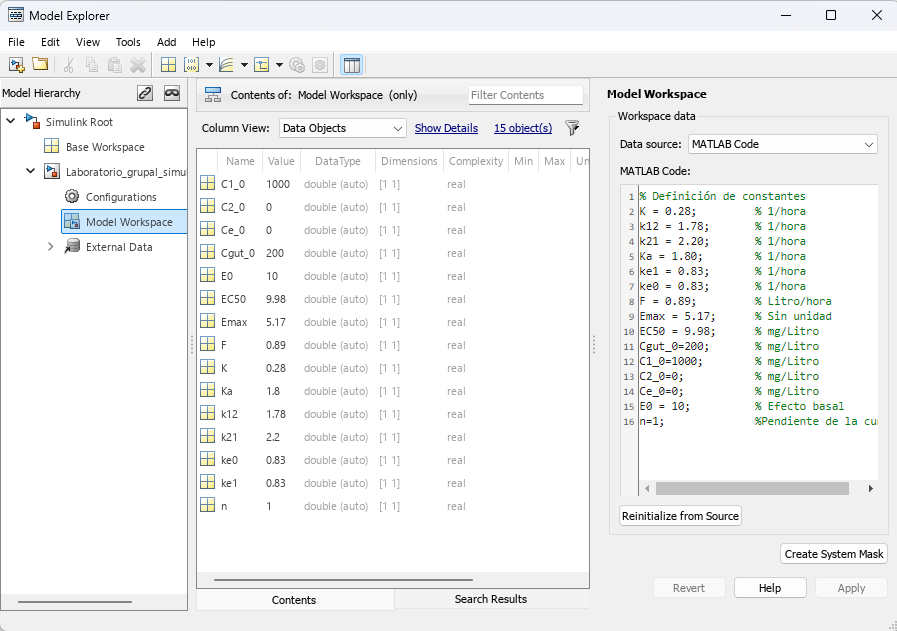
\includegraphics[width=0.75\linewidth]{Model_explorer.png}
\caption{\label{fig:Model_explorer}Definición de parámetros y condiciones iniciales en Model Explorer}
\end{figure}

El solver empleado es Runge-kutta de orden 4 (ode4), se ha utilizado un paso de integración de h=0.01 y un intervalo de tiempo de [0,8]. En este caso las constantes se dan en unidades de horas, por lo que el resultado de la ecuación diferencial será concentración por hora. Así, el límite de la simulación es 8 h. Se presenta en la la Figura~\ref{fig:Solver} una captura de pantalla realizada con la configuración del solver.

\begin{figure}[H]
\centering
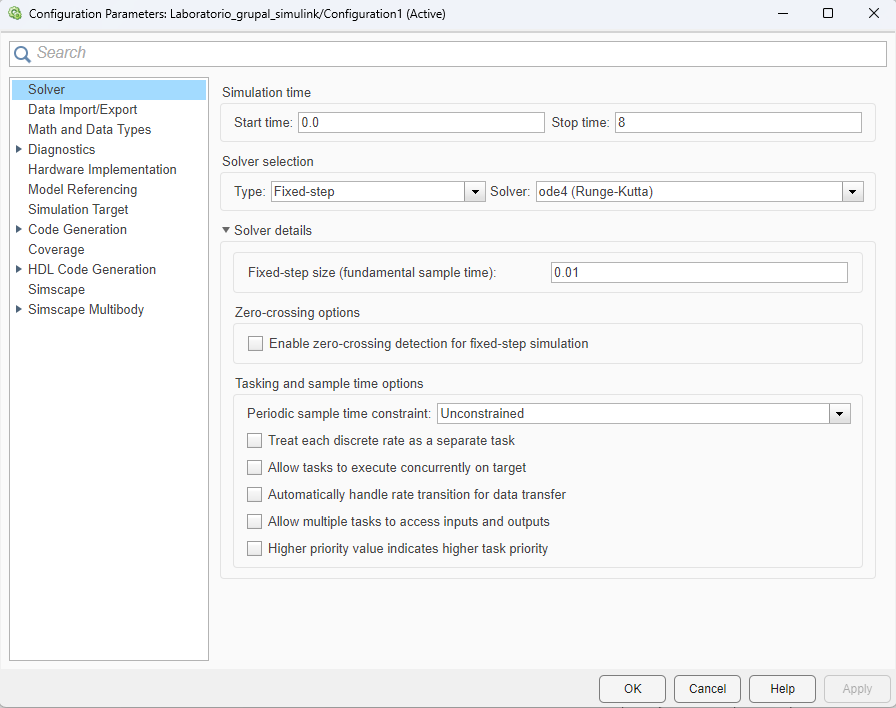
\includegraphics[width=0.75\linewidth]{Solver.png}
\caption{\label{fig:Solver}Características del solver empleado}
\end{figure}

\end{document}
